\documentclass[12pt]{article}
\usepackage{xeCJK}

\usepackage{charter}
\usepackage{fullpage}
\usepackage[colorlinks,linkcolor=blue]{hyperref}
\usepackage{ifthen}
\usepackage{comment}
\usepackage[title,titletoc]{appendix}
\usepackage{pagecolor}
\usepackage{amsmath}
\usepackage{amsfonts}
%\usepackage[normalem]{ulem}
\usepackage{siunitx}
\usepackage{amsthm}
\sisetup{per=slash, load=abbr}

\usepackage{pgfplots}
\usetikzlibrary{positioning}
\usetikzlibrary{fit}
\usetikzlibrary{snakes}
\usetikzlibrary{shapes.geometric}
\usetikzlibrary{patterns}
\usetikzlibrary{shapes,arrows,chains}
\usepgfplotslibrary{patchplots,colormaps}
\usetikzlibrary{calc}
\usetikzlibrary{positioning, fit}
\usetikzlibrary{backgrounds}
\usetikzlibrary{intersections}

\newcommand{\whitepaper}[1]{\begin{center}\fbox{\parbox{0.75\textwidth}{{\small
#1}}}\end{center}}

\newcommand{\pcolor}{white!25}

\usepackage{setspace}
\usepackage[ruled]{algorithm2e}
\bibliographystyle{ieeetr}

\usepackage{geometry}
\geometry{left=3cm,right=3cm,top=1.6cm,bottom=3cm,headheight=0pt,headsep=1.5em}
\usepackage{fancyhdr}
\pagestyle{fancy}
\chead{
\includegraphics[scale=0.2]{../common/Nebulas.png}}  %在此处插入logo.pdf图片 图片靠左
\lhead{} % 页眉中间位置内容
\rhead{}
%\setlength{\topskip}{1em}

\usepackage{indentfirst}





\setCJKmainfont[BoldFont = STSongti-SC-Bold]{STSongti-SC-Regular}
\setCJKfamilyfont{hei}{SIL-Hei-Med-Jian}		%宋体
\setCJKfamilyfont{song}{SimSun}		%宋体
\setCJKfamilyfont{kai}{Kaiti}		%楷体
\setCJKfamilyfont{fang}{song}	%仿宋
\setCJKfamilyfont{li}{song}			%隶书
\setCJKfamilyfont{you}{Yuanti}		%幼圆

\newcommand{\song}{\CJKfamily{song}}	%宋体
\newcommand{\hei}{\CJKfamily{hei}}	%黑体
\newcommand{\kai}{\CJKfamily{kai}}	%楷体
\newcommand{\fs}{\CJKfamily{fang}}	%仿宋
\newcommand{\li}{\CJKfamily{li}}		%隶书
\newcommand{\you}{\CJKfamily{you}}	%幼圆
\newcommand{\reffig}[1]{图\ref{#1}}
\newcommand{\refsec}[1]{\S \ref{#1}}

\onehalfspacing   % ----------设置1.5倍行距(可能有意义,待调整)

%\parindent=20pt  % -------------------首行缩进大小,英文分段就直接0pt了吧。
\setlength{\parindent}{2.1em}
\setlength{\parskip}{0.3\baselineskip}
\newcommand{\nrcore}{Core Nebulas Rank}
\newcommand{\nrext}{Extended Nebulas Ranks}
\newcommand{\dom}{{\; \texttt{dom}\;}}

\setCJKsansfont[BoldFont = STHeitiSC-Medium]{STHeitiSC-Light}


\newtheorem{property}{特征}
\newtheorem{corollary}{推论}
\newtheorem{lemma}{引理}
\newtheorem{theorem}{定理}
%\addbibresource{reference.bib}

\begin{document}
\pagestyle{empty}
\renewcommand{\contentsname}{目录}
\renewcommand{\abstractname}{摘要}
\renewcommand{\refname}{参考文献}
%\renewcommand{\nomname}{术语表(按首字母排序)}
\renewcommand{\figurename}{图}
\renewcommand{\tablename}{表}
\renewcommand{\baselinestretch}{1.5}
\renewcommand{\appendixname}{附录}
\renewcommand{\proofname}{证明}

\pagecolor{\pcolor}

\begin{titlepage}
  \begin{center}
    \vspace*{5.5cm}
    
\includegraphics[scale=0.5]{../common/Nebulas.png}
    \vspace{0.5cm}


    \textbf{\huge{Consensus Survey}}

    \vspace{0.5cm}
    星云研究院
    \vfill
    2019年2月 \\
    版本号:0.0.1
    \textbf{}
  \end{center}

\end{titlepage}
\setcounter{page}{0}
%\thispagestyle{empty}
\tableofcontents
\newpage
\setcounter{page}{1}
\pagestyle{fancy}                                 
\vspace*{0.01cm}
\section{介绍}
区块链技术在近十年来有了长足发展,其中,共识算法是区块链最为核心的技术之一。十年来,各式区块链项目如雨后春笋办冒出,也为我们带来了丰富多彩的共识算法及新的思考。

本文将从技术的角度对现在区块链行业热门的共识算法进行调研。相比于现有的共识算法调研如~\cite{wang2019survey,袁勇2018区块链共识算法的发展现状与展望},本文具有如下特点。

1.本文将以章节的形式,每一章节对一个共识算法进行着重介绍。在具体写作方面,本文将不拘泥于对共识算法进行传统意义上的分类,而是突出各共识算法在技术上的贡献以及在新的共识设计上能参考的点。我们认为,每个共识算法都有其独特之处,而传统意义上的分类(如去中心化程度,PoX之类)并不能很好的将其反映出来。

2.本文假设读者对最基本的共识算法,如PoW,PoS,BFT等有一定了解,不会做详细介绍。且本文主要作用是供内部设计共识参考用,故重点会放在对新共识设计的思考上。
\section{背景}
关于共识的研究最早可以追溯到1959年~\cite{eisenberg1959consensus}。计算机领域的共识主要研究分布式系统中所有节点达成一致性的问题。具体到区块链中的共识算法而言,其目的是决定出块权(及其奖励)的归属,需要满足下面两个基本性质。(各文献的描述存在细微差别)

\begin{itemize}
\item 一致性(consistency, safety)所有诚实节点最终(对某个提案)达成一致。
\item 活性 (liveness)所有诚实节点发起的交易最终都会被记录,
\end{itemize}
同时,一个好的区块链共识算法有如下基本指标:
\begin{itemize}
\item 去中心化:出块权不应集中在某个个体或团体手里。
\item 抗女巫攻击:鉴于在区块链上建立新账户是没有成本的,共识算法的模型应该能够遏制用户通过大量建立新账户来提升自己获得出块权的概率。PoW和PoS分别用算力以及才产作为竞争出块的依据来防止女巫攻击。
\item 每秒交易次数(TPS):TPS反映出区块链系统的吞吐量。目前比特币的TPS为10,以太坊为15-25。
\item 交易确认时间:交易确认时间影响链上交易的效率以及用户体验。目前比特币的确认时间为1小时,以太坊为3分钟左右。
\end{itemize}

\subsection{思考}
现在普遍认为区块链系统中也有不可能三角的存在,即去中心化,安全性和可扩展性不能同时达到。故设计新共识时需要有所取啥。

同时,女巫攻击以及去中心化(反独裁性)也难以同时保证。假设财产为$a(b)$的账户能产生的收益(由共识算法决定的,如出块奖励)为$f(a)(f(b))$。若能抵抗女巫攻击,理论上需要满足$f(a+b)>f(a)+f(b)$。这样可以推出$f(n)>nf(1)$,意味着大户的绝对统治($n$可以达到上亿级别)。

值得注意的是,上述分析不仅仅适用于PoS机制,即使是对PoW机制$f(a)$也可以理解为财产为$a$的用户的挖矿效用,因为两者存在正相关关系。所以现在的比特币也可以理解为被矿池所统治的中心化系统,但同时浪费了额外的资源进行挖矿。相比而言,PoS机制没有挖矿,但同时也是一个受资本操控的系统。

{\color{red}是否存在矿工证明和系统利益一致的共识?}

例如,矿工通过提升节点性能来挖矿,并且同时能够提升整个系统的TPS,但是这样可能造成安全性降低(见第二章,GHOST)。 或者通过吸引新用户加入来挖矿,但这样除了IOTA这种DAG系统之外,节点数目超出系统容量之后反而会降低系统性能。

其他思考:

是挖矿还是看资产?

是否要有委员会/准入门槛?

是否支持智能合约?

是否考虑分片?或者用DAG?


\part{对比特币扩容的思考}
\section{GHOST}
\subsection{介绍}
GHOST的全称是The Greedy Heaviest-Observed Sub-Tree,由Yonatan Sompolinsky和Aviv Zohar 在2015年提出。其主要思想是对比特币最长链原则的一种修改。\footnote{比特币工作量证明可能会出现两个矿工几乎同时发现新的合法区块的情况,当他们同时公布自己新挖出得区块并接在当前主链上,这样就产生了分叉。比特币Nakamoto共识约定当前主链存在多个分叉时,将最长(即区块高度最高的)的分叉链最为唯一合法的链。}	

GHOST实现的主要目标是,在保证安全性的前提下给出了比特币的扩容方案。该共识思想已经成为以太坊升级项目的一部分。

\subsection{模型}
众所周知,比特币中存在$51\%$攻击,即需要假设作恶节点所占的算力比例不超过一半。这个假设在各大共识算法中都普遍存在。但GHOST认为,在比特币系统实际运作中,作恶节点实际需要占据的算力比例不需要$50\%$那么多即可发起攻击。


GHOST用$tree(t)$表示在时刻$t$整个区块链的结构,(所有区块)。由于分叉的可能性,这个$tree(t)$不一定是一条链,而是“区块树”。
\begin{itemize}
	\item $\lambda_h$,表示诚实节点的出块速率,即新区快加入某个$tree(t)$的速率。值得一提的是,并不是所有的诚实节点出的区块都会最终出现在主链上,因为诚实节点之间也存在竞争,可能出现同时出块的情况进而产生分叉,
	\item $q\cdot\lambda_h,0<q<1$,表示作恶节点的出块速率。值得一提的是,作恶节点比诚实节点更团结——他(们)永远都只会在某一条秘密的链上进行挖矿,不会出现分叉。
	\item $s(T)$,$s$函数用于确定主链成员:输入一个子树$T$,输出一个区块,这个区块被确定为主链成员同时为下一个区块的父区块。比特币的最长链原则即让最长子链的起始区块作为$s$的返回值。
	\item $\beta$,表示主链增长的速度。注意只有$s$函数所决定的区块才能被主链记录。
	\item $TPS=\beta(\lambda,b)\cdot K$,其中$b$为区块大小(KB),K为平均每KB数据包含的交易数目。
\end{itemize}
在比特币最长链原则下,针对传统的$51\%$攻击,GHOST认为,{\color{red}需要竞争的是(诚实节点带来的)主链增长速度与作恶节点的秘密链的增长速度,即$\beta$与$q\cdot\lambda_h$,而不简单的是用出块速率$\lambda_h$来对比。}所以,GHOST把$\frac{\beta}{\lambda_h}$作为所谓的“安全系数”,即当且仅当$q>\frac{\beta}{\lambda_h}$时作恶节点将会成功攻击(传统认为需要$q>1$才能进行攻击)。
	
\subsubsection{对比特币扩容的思考}
比特币的低TPS一直是人们诟病的原因。两种简单的提升TPS的想法为:
\begin{itemize}
	\item 增加每个区块的大小。(增大$b$,比特币的区块平均大小为1MB)
	\item 减小区块出块的平均间隔时间。(增加$\lambda_h$,目前比特币的平均间隔为10分钟)
\end{itemize}
根据定义,咋看之下这两种方式确实能提升TPS,但{\color{red}GHOST指出这两中简单的方法都存在一系列问题。而这也是GHOST这篇论文的主要贡献。}

1.增加区块大小$b$

随着区块容量的变大,当矿工挖到新的区块时需要更长的时间来广播,同时用户也要花更长的时间来同步实时的区块链状态。这意味着新的区块需要花更长的时间被主链接收且被绝大多数节点验证,这样会导致更容易产生孤块,更容易发生分叉,安全性降低,主链增长速度反而会受到影响。有调研表明[]在维持基本的安全性的情况下比特币区块容量不能超过8M。

2.增加出块速率$\lambda_h$

注意到当$\lambda_h$增加时,直接影响是安全系数$\frac{\beta}{\lambda_h}$降低了。原因是诚实节点和作恶节点的出块速率都会增加,同时也会造成状态同步压力变大,分叉变多,主链增长速率$\beta$的提升受限。

所以,GHOST对简单的通过增加区块大小和降低出块时间的比特币扩容进行了否定。

\subsection{GHOST算法}
如前所述,GHOST的核心思想是将比特币的最长链原则改为最重子树原则。

对一个区块$B$,定义$subtree(B)$为以$B$为根的子树,$Children(B)$为$B$的直接子区块。写下来我们将实现GHOST中的$s$函数,用于决定一棵树被选为主链的块。

\begin{algorithm}[H]
	\caption{GHOST}%算法名字
	\KwIn{Block Tree $T$}
   set $B \leftarrow Genesis Block$\;
	\eIf {$Children(B)=\emptyset$}
    {Return $B$ and exit\;}
   {Update $B\rightarrow \arg\max_{C \in Children(B)}|subtree(C)|$\;}
	GOTO line 2\;
\end{algorithm}
其核心思想如\reffig{fig:GHOST1}(1B,2C,3D这几个区块相比其兄弟区块拥有更重的子树。)
\begin{figure}
	\centering
	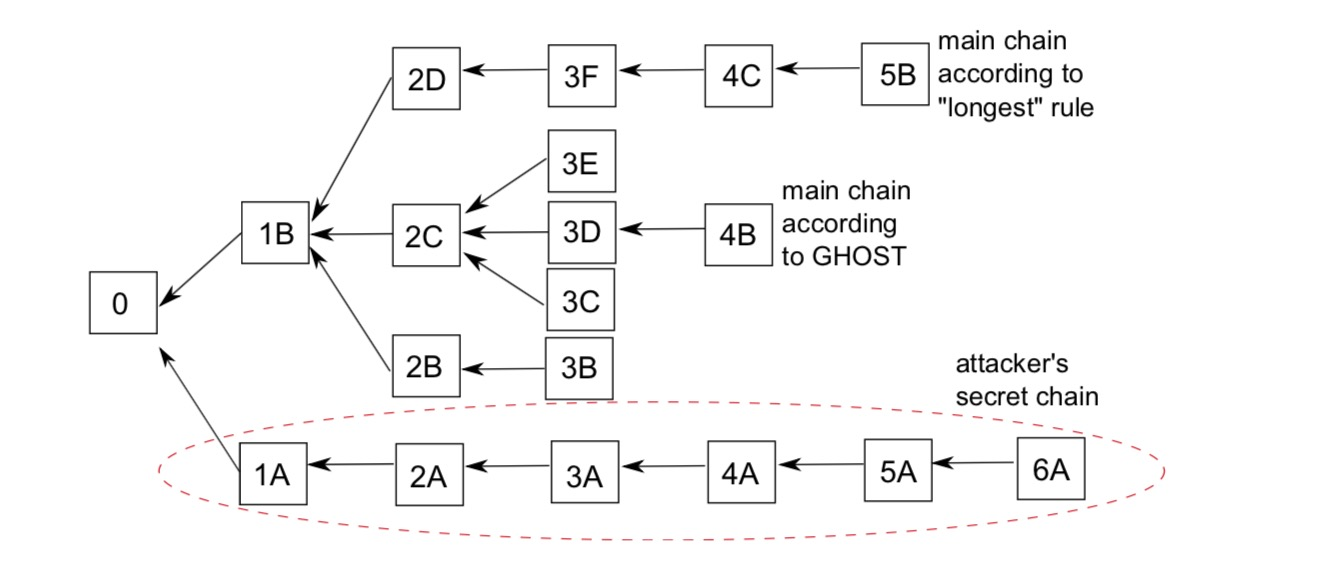
\includegraphics[width=1\textwidth]{../common/GHOST_1.png}
	\caption{GHOST中的最重子树} 
	\label{fig:GHOST1}
\end{figure}


\subsection{性质分析}
相比于比特币的最长链原则,GHOST的主要性质是安全系数能独立于区块产生的速度,始终为1(即能抵抗$50\%$的攻击)。这个性质由下面两个引理保证:
\begin{lemma}
	定义$\psi_B$为区块$B$或者被所有节点接受,或者被所有节点所拒绝的时刻。那么$Pr(\Psi_B<\infty)=1$且$E[\Psi_B]<\infty$
\end{lemma}
即这个引理保证最终一致性。和比特币一样,GHOST不存在finality状态,故这个一致性也是概率上的。这个引理的证明思想是,出现不一致性仅当存在两个重量相同的子树。那么存在一个时刻,在一段时间内只挖出一个区块且在之后进行广播的过程中也没有新的区块被挖出,那么平衡将被打破,最重子树得以确定。

GHOST的抵抗$50\%$以下攻击由下面的引理决定:
\begin{lemma}
	如果$0<q<1$,假设区块$B$已经在主链上出现的时间趋于无穷大,那么它被排出主链的概率趋近于0。
\end{lemma}
由于这个结论与$\lambda_h$无关,这就为GHOST的扩容提供了保证。下面两张图给出了GHOST的TPS及安全系数随$\lambda_h$的变化。

\begin{figure}
	\centering
	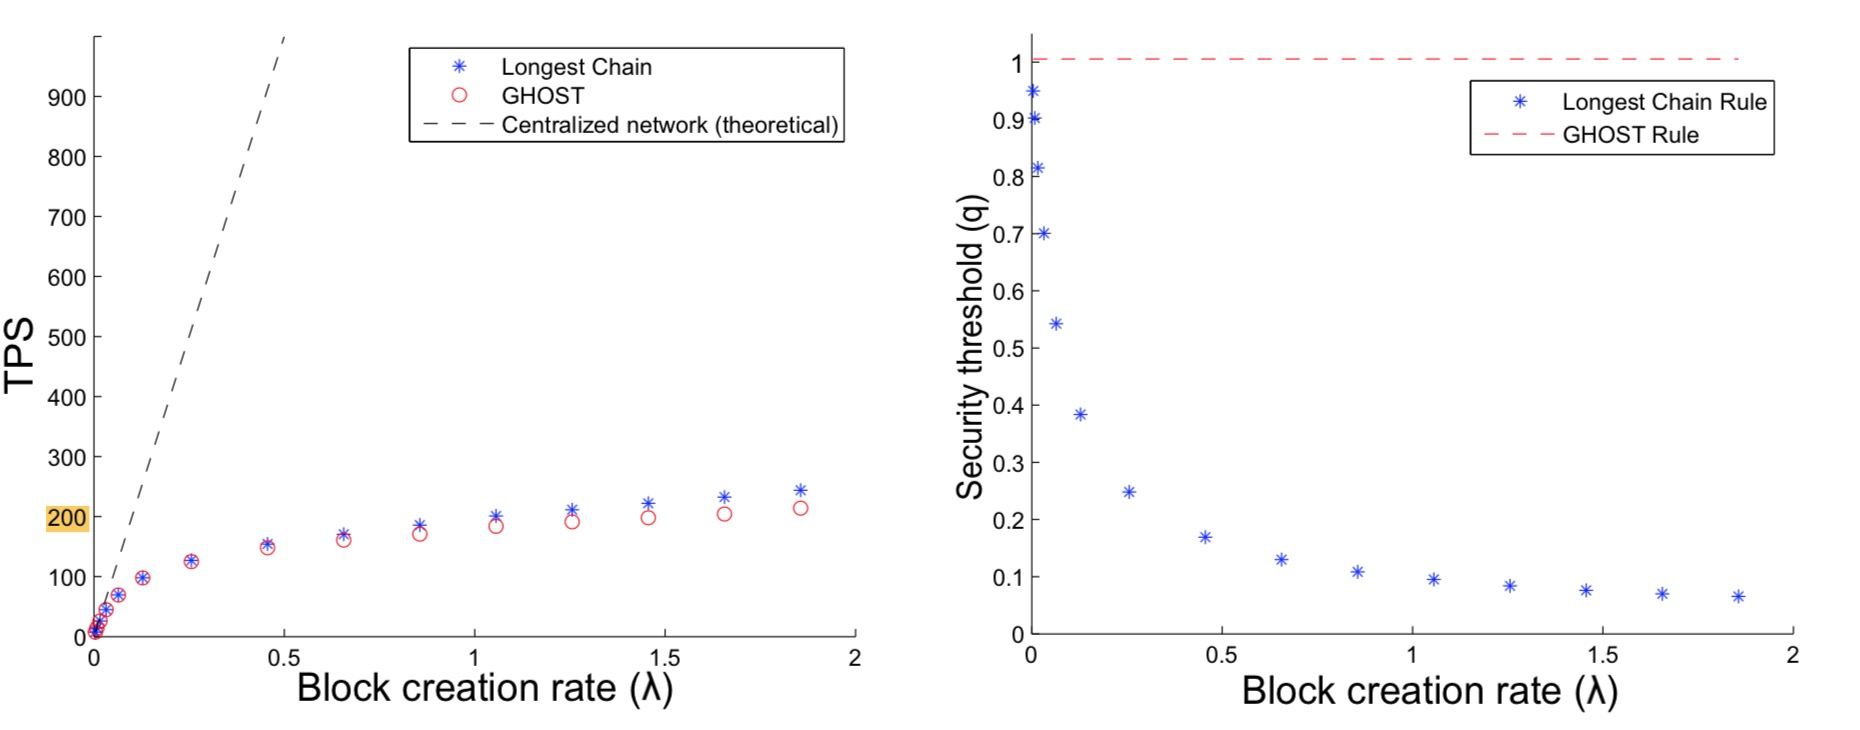
\includegraphics[width=1\textwidth]{../common/GHOST_2.png}
	\caption{TPS与安全系数的变化} 
	\label{fig:GHOST2}
\end{figure}

所以,当$\lambda_h$达到一定数值后TPS可以达到200左右,若再继续增大整个系统的同步会受影响,安全性降低,故对主链增长及TPS的提升很小。

文章最后还有一些关于主链增长速度的定理。这里不做详细介绍。
\subsection{总结}
GHOST给我们最大的其实是不能简单地靠增加出块速率和区块大小来增加TPS。设计共识算法是可以不局限于最长链原则。


	


\section{Bitcoin-NG}
\subsection{介绍}
Bitcoin-NG是另一个针对比特币的扩容限制(scalability limits)提出思考的论文,发表在NSDI16上~\cite{eyal2016bitcoin}。其作者之一Ittay Eyal专攻区块链与博弈论相结合的领域,曾提出过私自挖矿(selfish mining~\cite{eyal2018majority})等著名进攻方式。该论文提出基于比特币的扩展协议旨在满足下面的目标:
\begin{itemize}
	\item Bitcoin-NG的延迟只受限于网络传输的延迟。
	\item Bitcoin-NG的带宽只受限于个人节点的处理容量。
\end{itemize}

\subsection{模型}
其主要思想是,允许矿工在挖出一个(主)区块的基础上,按固定速率不断出接在主块之后的子区块(microblocks),直到下一个主区块被挖出。这段时间内这个矿工叫做leader,而只有包含leader有效签名的子区块才会被认可。子区块无需工作量证明,但产出子区块的速率被事先确定。

\begin{figure}
	\centering
	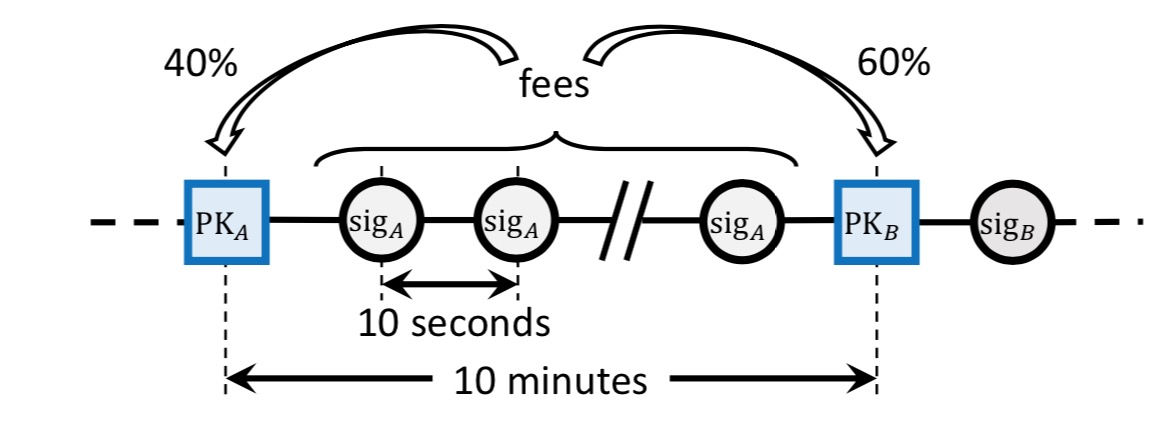
\includegraphics[width=0.7 \textwidth]{../common/BTCNG_1.png}
	\caption{Bitcoint-NG区块结构。其中$40\%$和$60\%$分别为一个子区块的交易费的分配方式,即leader获得$40\%$,挖出下一主块的矿工获得$60\%$} 
	\label{fig:BTCNG1}
\end{figure}
\reffig{fig:BTCNG1}展示了Bitcoin-NG的区块结构以及交易费的分配方式。

值得注意的是,因为每个leader都会尽全力出子区块,所以,当下一个主区块被挖出的时候几乎会必定产生分叉,如图\ref{fig:BTCNG2}。所以,文章指出当用户收到一个子区块的时候,在确认该区块在主链之前应该等一段时间。
\begin{figure}
	\centering
	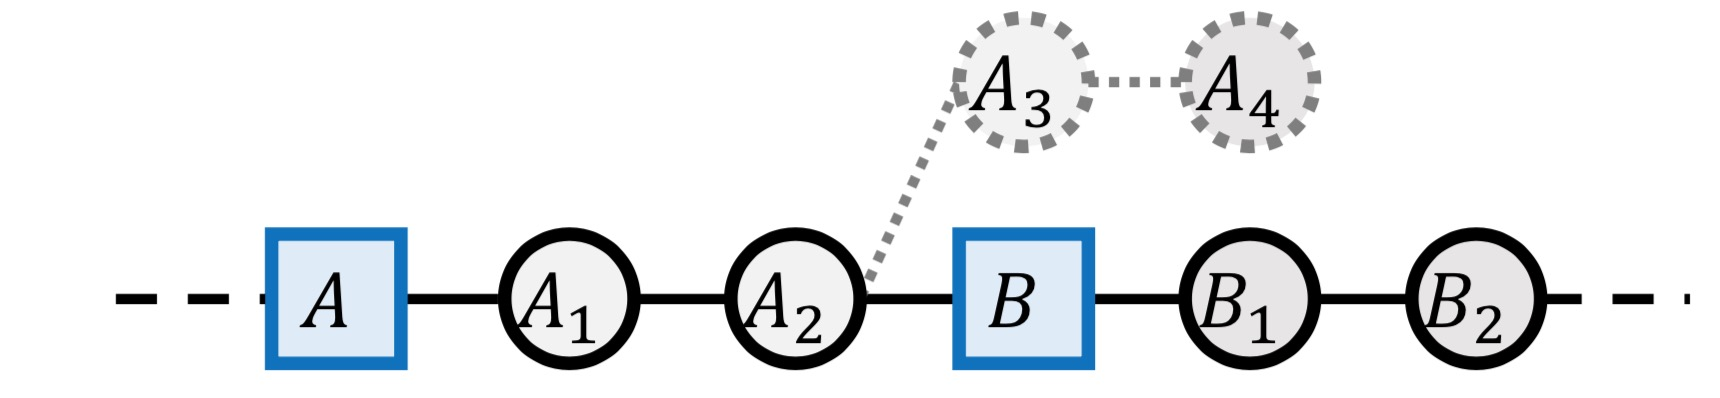
\includegraphics[width=0.7	\textwidth]{../common/BTCNG_2.png}
	\caption{Bitcoint-NG分叉情形:leader $A$一直在出子区块,但是矿工$B$已经在子区块$A_2$后面挖出了一个主块。} 
	\label{fig:BTCNG2}
\end{figure}

同时,因为每个leader拥有自块的任意出块权,他可以选择恶意分叉他出的子区块以实现双花攻击(double spending)。Bitcoin-NG的解决方式是,允许任何用户发送一个有毒交易(poison transaction),这个有毒交易是对分叉行为的一种举报,包含被裁减的分叉的第一个区块的内容,作为“欺骗证明(proof of fraud)”。每个leader需要等待一定的时间(maturity window)才能获得发区块的收益,在这期间内一旦被举报作弊leader将失去收益作为惩罚。同时,发出有毒交易当前leader能获得作弊者赔偿的$5\%$。

\subsection{安全性分析}
Bitcoin-NG假设作恶节点的比例不超过1/4。这是在考虑到了私自挖矿(selfish mining~\cite{eyal2018majority})的情况下。鉴于大量其他共识的论文并没有把私自挖矿考虑进去,这里不做详细介绍。

文章接下来从博弈论角度分析leader的进攻方式。假设每笔交易费有$r_{leader}$(待定)的比例归leader所有,剩下$1-r_{leader}$归挖出下一个区块的矿工所有。假设leader拥有全网$\alpha$比例的算力:
\begin{itemize}
	\item 当leader创建包含某笔交易的子区块时,他不公布这个区块,而是在这个区块之后继续挖矿,期待自己能挖到后继的子区块,这样能获得该笔交易$100\%$的交易费。若失败,该笔交易被部署在其他矿工挖出的子区块上,则该leader回归正常,继续在新的子区块上挖矿。这种行为不会提升该leader的收益当且仅当
	$$ \overbrace{\alpha\times 100\%}^{Win}+\overbrace{(1-\alpha)\times\alpha \times ( 100\%-r_{leader})}^{Lose~but~mine~after~txn}<r_{leader}$$
	当$\alpha<1/4$时,解得$r_{leader} >37\%$
	
	\item 对于某笔交易,leader选择裁减掉这笔交易所在的区块,直接在其之前的区块上挖矿。若leader成功挖出下一个主区块,则他可以将该特定交易部署到自己接下来出的子区块上,并继续挖矿争取能挖到再下一个主区块以获得该笔交易的剩余交易费。相比于直接在这笔交易子区块挖矿,leader的收益不会提升当且仅当
	$$ \overbrace{r_{leader}}^{Place~in~microblock}+\overbrace{ \alpha \times ( 100\%-r_{leader})}^{Lose~but~mine~after~txn} < 100\%-r_{leader}$$
		当$\alpha<1/4$时,解得$r_{leader} < 43\%$
\end{itemize}
故$r_{leader} = 40\%$ 是一个可行的选择。

作为一个博弈论专家,作者接下来考虑的是各种可能的进攻方式以及各类指标(比通常的共识算法考虑的更多)并与比特币进行比较。这里列出一些重点供参考。

1.关于挖矿难度:比特币的挖矿难度是动态调整的,故矿工有动机在难度较高的时候停止挖矿或转向其他公链挖矿,等到难度降低之后再回归。而在Bitcoin-NG中,由于子区块的出块速率是固定的,故只有主区块会受到这种行为的影响。故相对而言影响较小。

2.关于分叉。Bitcoin-NG承认会比比特币拥有更多的分叉,如\reffig{fig:BTCNG2}所示。但是,在Bitcoin-NG中分叉消失的更快,因为一旦一个主区块被挖出则leader权改变,子区块分叉消失。但是对于主区块的分叉并没有解释很清楚。(见原文5.2)

3.文章提出了一些衡量区块链性能的指标,包括共识延迟,公平性,矿力利用率,修剪(分叉被确认忽略)时间,	胜利(主链确认)时间等。文章的实验是基于不同的区块大小和出块评率绘制上述指标的曲线,并与比特币相比较。有兴趣的读者可以参阅原文查看结果。

\subsection{总结}
Bitcoin-NG这种出小块的思想具有一定的借鉴意义,类似于一种锦上添花的功能,但和GHOST一样,对共识原型的贡献不大。同时,文章并没有很显示的证明本章节开头提出的关于比特币扩容的两点。另外,文章提出的各项指标实际被后续工作引用的不多,参考价值有限。


\part{少量节点的强一致性保证:BFT}
\section{BFT背景:拜占庭将军问题}
BFT(Byzantine Fault Tolerance的全称是拜占庭容错,是一个能实现状态机复制且能够容忍拜占庭节点的算法。这里的拜占庭节点的就是所谓的恶意节点,其行为可以是任意的(发送错误信息,任意长时间不响应信息,不按照协议运作等等,且各个拜占庭节点之间可以合谋)。

介绍BFT要从广为人知的拜占庭三将军问题(BGP,Byzantine General Problem)说起。这两者容易混淆,但实际BFT指的是一系列容错问题,而BGP是BFT的一个特例。

BGP问题由Lamport在1982年提出\cite{lamport1982byzantine}。所谓三将军BGP问题指的是,有一个指挥官和两个将军,他们需要对进攻或者撤退达成统一的决定,其中他们之间有一个叛徒,这个叛徒就是我们之前提到的拜占庭节点,可以任意行为(如撒谎,不回复等)。
将军们(包括指挥官)之间可以任意轮进行点对点交流。问题要求,如果指挥官是诚实的(不是叛徒),那么所有诚实将军的决定要和指挥官的决定一致。如果指挥官是叛徒,那么所有的将军要做出一致的决定。

常规的BGP问题分为两个部分,分别针对\textbf{同步网络模型}和\textbf{异步网络模型}。

同步网络:所有节点的消息传输的延迟不会超过某个定值$t$(这个$t$是有限且已知的)。

异步网络:所有节点的消息传输延迟可以是任意的(对于诚实节点的只能保证消息一定可达,但是延迟上限未知,且随时间是可变的)。

同步网络是一种理想的网络环境,而我们熟知的BGP在同步网络环境的描述如下:

\textbf{同步网络环境下三将军BGP问题不可解,四将军或以上BGP问题可解}

这个问题的证明是如果指挥官是恶意的,那么他可以给两个将军发出不同的指令。如果指挥官不是叛徒,那么两个将军交流时其中一个将军可以谎报指挥官的指令。具体细节这里不介绍,可以参阅知乎专栏\cite{zhihuBFT}。值得注意的是这里的不可能与后面提到的FLP没有关系,因为是同步网络环境,仅由数学上的推导即可得出。

这个问题(同步BGP)在四将军(包括指挥官)情况下是有解的。同时可以推广为,假设拜占庭节点 (将军)的数目为$f$,当且仅当将军总数大于等于$3f+1$时BGP问题是有解的。

当然对于同步三将军BGP,Lamport提出的解决方案就是加入签名\cite{lamport1979constructing},加入了签名之后,即便全世界只有两个将军是诚实的而其他将军全是叛徒,这两个将军也能达成共识。这其实就是前段时间疯传的V神发现了$99\%$共识算法。

\textbf{异步网络环境下BGP问题无解}

如前所述,异步网络环境下消息传输延迟可以使任意长且可变。这种情况下只要存在一个叛徒BGP问题就无解。这是由分布式系统的经典结论,FLP不可能定理得出\cite{fischer1982impossibility}。主要原因当一个节点长时间未接收到消息时,他无法判定对方是恶意节点故意不发还是对方是诚实的但因延迟消息还未传过来。书\cite{wattenhofer2016science}第三章有对FLP问题的详细证明。	

这里注意到拜占庭节点“不说话”事实上在异步BGP问题中更具杀伤力,因为有了签名的存在,任何节点能伪造的信息有限(容易被查出),而“不说话”让其他节点无法分辨是恶意节点还是消息没达到。退而求其次的,人们开始在给定某些假设的情况下研究BGP问题:假设指挥官一定会发信息(可以说假话,但一定会到达),且可以引入签名,这种情况下三将军BGP能不能解决。这种假设在\cite{zhihuBFT}叫“弱终止假设”(或者可以理解为半异步假设。这个假设仅仅针对BGP问题,在实际中并不常见)

\textbf{弱终止假设环境下三将军BGP问题无解,四将军或以上问题有解}

同样,该结论可推广为当且仅当$3f+1$或以上将军可解。

BGP的结论总结如下:

\begin{tabular}{|c|c|c|c|c|}
环境	& 同步(无签名)& 同步(带签名)& 异步  & 弱终止 \\\hline
有解所需最少将军数 &  $3f+1$ &   2   &   $f>0$必无解  &    $3f+1$ \\    
\end{tabular}
\section{PBFT}
\subsection{背景}
BGP问题是BFT问题的一个特例:他假设所有节点对指挥官的身份形成了共识。实际的BFT问题里不一定有指挥官的存在,但拜占庭节点仍然存在。以下用$f$表示拜占庭节点的数量,用$n$表示总结点数量。解决问题的思路仍是沿用BGP问题的解法。

上一章我们提到了同步模型与异步模型的概念。这里指出,当我们研究区块链的共识算法的时候,鉴于区块链的大规模和去中心化,我们希望基于的都是异步模型的假设。现在的各项文献同步模型的研究已经不多。

然而异步环境共识不可避免的受限于FLP不可能定理:
\begin{theorem}
	当$f>0$,不存在一个确定的算法总能在异步网络环境下达成共识。
\end{theorem}
所以,各大著名的异步共识算法实际都做了各式各样的假设。如Ben-Or算法~\cite{ben1983another}引入随机性,即一定情况下需要节点各自通过掷硬币来选择决定,同时期望若干轮后所有诚实节点能掷出同样的结果。该算法仅能容忍$f<1/10n$的拜占庭节点,同时达到共识的期望轮数是指数级别。类似共享硬币~\cite{bracha1987asynchronous}的思路能够提升时间复杂度,但容错率仍然很低。

在正式介绍PBFT之前,我们这里简单介绍状态机复制,指的是一系列节点(初始状态相同)以相同的顺序执行一系列指令的问题。这个要求实际上比共识更强,因为像现在如比特币的共识是概率性的,即很难被扭转,但并不存在所谓的Finality状态,即完全一致性。而状态机复制需要保证完全的一致性。另外,如果一个算法能实现状态机复制(可能各文献说法会有不同,但这里我们默认状态机复制已经满足一致性),则可由该算法实现共识问题。

\textbf{为什么要用PBFT?}

最初,Paxos[]算法的提出解决了同步网络下没有拜占庭节点的状态机复制问题。然而,在区块链被提出之前,PBFT等一系列实现异步状态机复制的算法并没有受到重视。其原因是在传统的中心化系统中,对指令时序的一致性要求并没有那么强烈,往往会根据具体业务实现不同层面的一致性和安全性指标——一般而言,双机备份就足以满足大部分业务需求,同j时大部分情况下少量指令顺序的改变并不会对最终结果产生太大的影响。

区块链的诞生让尘封已久的BFT重建天日:由于区块链的大规模以及去中心化(意味着难回滚,不可篡改,冲突难以调和,需要备份的节点多)特性,人们需求一个状态机复制的强一致性保证。而其中最著名的算法就是PBFT,其全称为Practical Byzantine Fault Tolerance~\cite{castro1999practical},发表在1999年OSDI上。

\subsection{模型介绍}
传统的状态机复制算法或者依赖于同步网络环境的假设,或者在实际运行时间太慢。PBFT旨在提出能实现$1/3$异步拜占庭容忍的确定性协议,用于实现服务器副本按顺序执行一系列操作的问题。论文的假设是,在任何时刻$t$消息传输延迟$Delay(t)$不会无限制增长。这是一个非常弱的假设,在实际中通常是满足的。而这个假设的存在导致PBFT算法和FLP定理并不矛盾。

定义$\mathcal{R}=\{0,1,...,|\mathcal{R}|\}$,其中$|\mathcal{R}|=3f+1$。PBFT将所有服务器分为一个主节点和其他副本节点。每个节点在他的视角看到的信息称为一个view,每个节点的view允许不同。一般而言,主节点由$p=v mod R$决定,其中$v$表示view的轮数,在算法里会不断更新。

大致而言,PBFT算法执行包涵下面4个步骤:
\begin{itemize}
	\item 客户端向主节点发送一个操作请求
    \item 主节点向所有副本节点广播这个请求
    \item 所有副本节点执行这个请求,并且给客户端发送一个带执行结果的回复(reply)
    \item 当客户端收到至少$f+1$个相同的回复时,即得到该操作请求的执行结果。
\end{itemize}

客户端等待f+1个从不同副本节点得到的同样响应,同时需要保证签名正确,并且具有同样的时间戳t和执行结果r。这样客户端才能把r作为正确的执行结果,因为失效的副本节点不超过f个,所以f+1个replicas的一致响应必定能够保证结果是正确有效的。

如果客户端没有在有限时间内收到回复,请求将向所有副本节点进行广播。如果请求已经在副本节点处理过了,副本节点就向客户端重发一遍执行结果。如果请求没有在副本节点处理过,该副本节点将把请求转发给主节点。如果主节点没有将该请求进行广播,那么就有认为主节点失效,如果有足够多的副本节点认为主节点失效,则会触发一次view change,即主节点轮换。

对于一个客户端而言,在他的视角内仅仅的是简单的发送一个请求以及接受多个回复的过程。所以PBFT的核心部分在于服务器节点之间的交互,被分为三个部分:\emph{pre-prepare, prepare, commit}。见~\reffig{fig:PBFT1}。
\begin{figure}
	\centering
	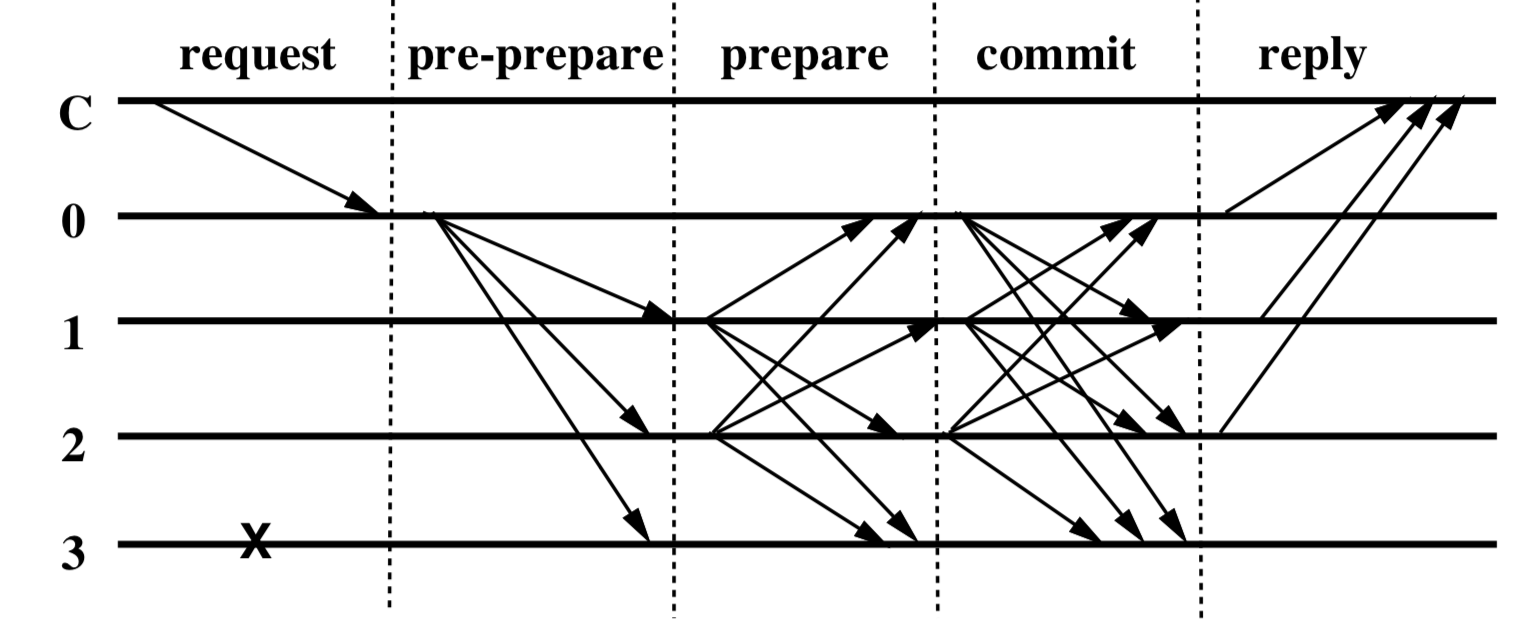
\includegraphics[width=1\textwidth]{../common/PBFT_1.png}
	\caption{PBFT流程} 
	\label{fig:PBFT1}
\end{figure}
\begin{itemize}
	\item \emph{pre-prepare}: 主节点分配一个序列号$n$给收到的请求($m$),然后向所有子节点广播pre-prepare消息$+m$,同时将请求消息$m$写入消息日志。消息的格式为$<PRE-PREPARE,v,n,d>_{\sigma_p},m>$,这里$v$是视图编号,$m$是客户端发送的请求消息,$d$是请求消息$m$的摘要(摘要在文章中的意思即哈希值$D(m)$,密码学上难以做逆运算),$\sigma_p$为主节点$p$的签名,$n$是消息的序号,必须在$h$和$H$之间(称为水线(watermark)限制这样可以防止拜占庭节点使用很大的$n$消耗序号空间)。注意为减少传输开销,此处客户端的原始请求并没有包括在pre-prepare消息内。副本节点只会接受格式,签名,view,水线限制均满足的pre-prepare消息。
	
    \item \emph{prepare}: 一旦副本节点接受了$<PRE-PREPARE,v,n,d>,m>$,则进入prepare阶段,同时。该节点向所有副本节点发送准备消息$<PREPARE,v,n,d,i>_{\sigma_i	}$,并且将两者写入自己的消息日志。定义$prepared(m,v,n,i)$为真当且仅当副本节点$i$已将下列消息写入日志:消息$m$,针对$m$且view为$v$且序号为$n$的pre-prepare消息,$2f$个从不同副本节点发来的与pre-prepare消息匹配的prepare消息。预准备阶段和准备阶段确保所有正常节点对同一个视图中的请求序号达成一致。预准备阶段和准备阶段确保所有正常节点对同一个视图中的请求序号达成一致,即$prepared(m,v,n,i)$和$prepared(m',v,n,j)$不能同时为真(若$m\neq m'$)。
    
    \item 当$prepared(m,v,n,i)$为真的时候,副本节点$i$将$<COMMIT,v,n,D(m),i>$向其他replicas广播,于是就进入了确认阶段。此阶段定义了两个函数,$committed(m,v,n)$为真的条件为:存在$f+1$个正常副本节点集合中使得其中所有副本节点$i$的$prepared(m,v,n,i)$为真。$committed-local(m,v,n,i)$为真的条件为:$prepared(m,v,n,i)$为真,并且$i$已经接受了$2f+1$个commits(包括自身在内)与pre-prepare消息一致。commit与pre-prepare消息一致的条件是具有相同的视图编号、消息序号和消息摘要。对某个正常节点$i$来说,如果$committed-local(m,v,n,i)$为真则$committed(m,v,n)$	也为真。这个不变式和视图变更协议保证了所有正常节点对本地确认的请求的序号达成一致,即使这些请求在每个节点的确认处于不同的视图。更进一步地讲,这个不变式保证了任何正常节点的本地确认最终会确认至少$f+1$个的正常副本。
\end{itemize}
视图变更协议:	所谓视图变更即将$v$加1,进而更换主节点。视图变更协议在主节点失效的时候仍然保证系统的活性。视图变更可以由超时触发,以防止副本节点无期限地等待请求的执行。

如果仅仅是这样,这个拜占庭容错在异步系统中是无效的。因为这个算法会在延迟超过阈值$t$的时候失效,而异步系统的定义就是找不到这样一个阈值$t$。PBFT采用的方法是:在$p=1$的时候,把阈值设为$t_1$,然后如果超时,则增加这个阈值。这样保证无论这个系统的延迟有多大,\emph{只要延迟不会无限增长},PBFT都能保证最终达成共识。

论文最后证明PBFT的安全性(safety)与活性(liveness),并进行了实验测试性能。这里不详细介绍,有兴趣的读者可以参阅全文。

\subsection{思考}
PBFT的好处是能够实现异步一致性,并且已经被大量区块链主要是联盟链项目所采用。其缺点在于共识的达成用到了长达三轮的消息传播,相对较长。在节点数量较少的情况下仍不失为一种最优的选择。

\section{投机BFT:Ouroboros-BFT与Zyzzyva}
对BFT的高通信复杂度优化的思考引出了一系列所谓投机BFT算法,即,在更强的假设前提下(网络环境更好或拜占庭节点更少)能有更好的性能(performance)。
\subsection{Zyzzyva}
Zyzzyva\cite{kotla2007zyzzyva}由Lorenzo等人在2007年提出,发表在SOSP上并被评为Best Paper。这个命名据说是选取的字典表里的最后一个单词,意味着Zyzzyva是这一系列算法的终结(然而之后还是出现了更好的算法)。

Zyzzyva的协议分为检查点(checkpoint)协议,视图转换(view change)和一致性(agreement)协议。这里我们介绍后两部分。

Zyzzyva其大致结构和定义和PBFT类似,($f$个拜占庭节点,一共$3f+1$个节点,异步网络模型)实现的目标是能有更快的消息复杂度,其核心思想在于在请求的确定被完全确定之前就开始执行。
\subsubsection{流程}
\begin{itemize}
	\item 1. 客户端发送请求给主节点
	\item 2. 主节点接受到请求,给其设置编号,并将请求广播到所有副本节点。
	\item 3. 副本节点接收到有序(ordered)请求,并投机的执行它们,并且给客户点发送回复。
	\item 4. 客户端开始接受副本节点发出的回复,根据\emph{一定时间内}收到的回复数量可以分为下面三种情形:
	   \begin{itemize}
	   	    \item 4a. 若客户端收到$3f+1$个回复(和他的请求匹配的),则认为请求被成功执行,完成请求(complete the request)
	   	    \item 4b. 若客户端收到的回复个数在$2f+1$和$3f$之间,则其生成一个commit信息(包含发送这$2f+1$个回复的节点的ID,签名,请求内容等),并广播给所有的副本节点
	   	        \begin{itemize}
	   	    	\item 4b.1 当副本节点接收到一个合法的commit信息时,生成一个local-commit信息并发送给客户端(若收到的commit信息包含的记录和本地记录不一致,则发起view change(更换主节点))
	   	    	\item 4b.2 当客户端收到$2f+1$个合法的local-commit信息时,完成请求。系统能保证即使存在view change,所有诚实的副本节点都会执行请求。(若客户端在限定时间内没有收到$2f+1$个local-commit信息则跳入4c步骤)
	   	    	\end{itemize}
	   	    \item 4c. 若客户端收到的回复个数少于$2f+1$个,则客户端将请求重新发送给所有副本节点并抄送给主节点(以获得序号)。
	   	     \begin{itemize}
	   	    \item 4c.1 当副本节点收到客户端的请求信息时,若该请求拥有最高的时间戳(timestamp),	则副本节点再发送一个confirm-req信息给主节点$p$并开始计时。若在限定时间内收到主节点发送的有序请求(order-req),则如前所述正常执行该请求。若在限定时间内没有收到,则发起view change,同时将confirm-req广播到所有副本节点。\footnote{注意到这里出现了$n^2$级别消息传输复杂度。}副本节点收到confirm-req时向发送方发送从主节点发来的有序请求。
	   	    \item 4c.2 当主节点收到confirm-req信息时,主节点如第二步所述发送有序请求。
	   	    \end{itemize}
	   	    \item 4d 当客户端发现请求不一致时,发送proof-of-mistake(POM)给所有副本节点并开始view change。(文章提到发起view change并不会影响请求被执行)
	   	\end{itemize}	
\end{itemize}

Zyzzyva的视图转换协议运作当且仅当下面两种情况发生
\begin{itemize}
	\item 当主节点查出有拜占庭行为
	\item 当$f+1$个节点发起view change(文中的方式为发送i-hate-the-primary信息)
\end{itemize}
\reffig{fig:zyzzyva1}演示了Zyzzyva的一致性流程。

\begin{figure}
	\centering
	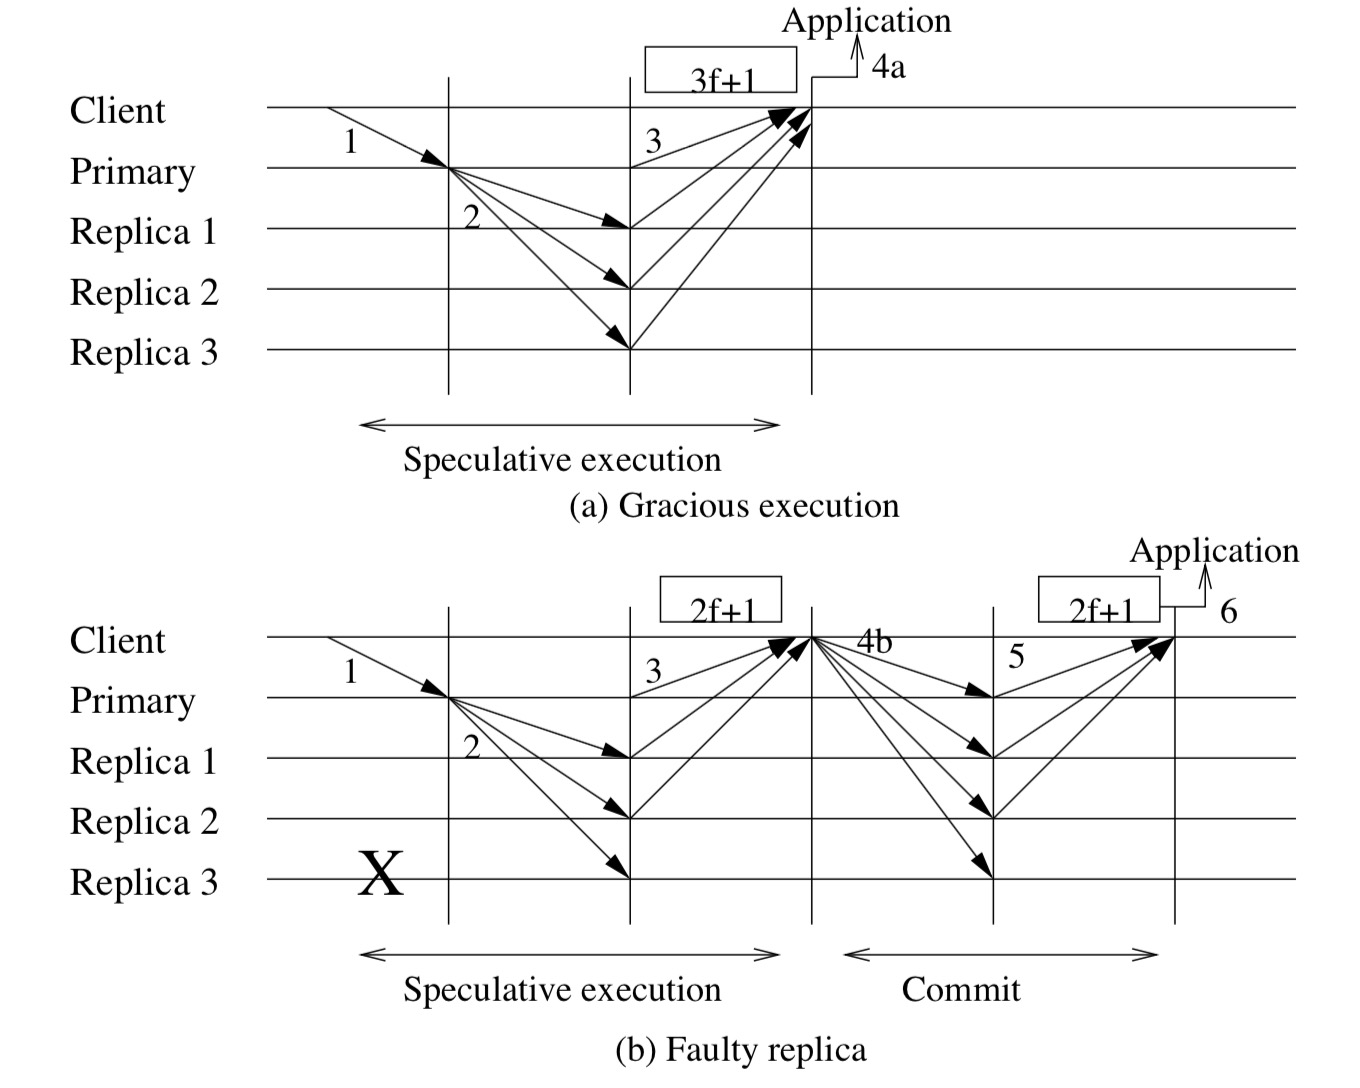
\includegraphics[width=1\textwidth]{../common/zyzzyva_1.png}
	\caption{TPS与安全系数的变化} 
	\label{fig:zyzzyva1}
\end{figure}

文章之后给出了安全性及一致性的证明,以及用实验对比PBFT的性能。这里不详细介绍。

\subsubsection{总结}
Zyzzyva和PBFT相比,运气好的时候执行的更快,但是当主节点更换频繁时效果可能更差。

值得一提的是,Zyzzyva团队之后又提出了致力于在更多的拜占庭故障发生时也能保持高性能的算法,发表在2009年NSDI上,称作Aardvark,据说是字典表的第一个单词(表达他们已经经历了一个轮回)。


\part{基于VRF的POS机制}
如果说工作量证明(Proof of Work)存在一个最为可能的替代品的话,那无疑是广为人知的权益证明(PoS)。对PoS的基本概率这里不多做介绍。值得一提的是,目前有个很大的误区是以太坊用的就是PoS机制,这个说法并不准确。以太坊现在的Casper~\cite{buterin2017casper}版本在出块方式上仍用的PoW,即挖矿机制。只有每隔50个区块需要通过委员会抵押投票的方式来确定一个检查点(checkpoint)以实现最终确认性(finality)。(成为委员会成员需要调用特殊的智能合约并抵押至少1500ETH,一个检查点需要有抵押总财富的2/3以上才能被最终确认)

所以,所谓的PoS目前解决的并不是由谁出块的问题,而是解决出完块后投票确认的问题。所以,在一系列PoS相关的文献里,出块权可以不做限定,而投票过程其实是另外一种达成共识的过程,可以与也可以不与所持财富(Stake)挂钩。本部分介绍的三大类似机制,Dfinity,Algorand和Ouroboros,都符合上述要求。这类文献为我们设计基于投票的共识机制提供了参考。

\section{Dfinity}
Dfinity是2018年在arxiv上的一篇论文,但作为代表引起了广泛关注。其本质做的是一个基于认证的联盟链,一切共识协议均根据可验证随机函数(Verifiable random function)实现,具有较快的传输复杂度(基本线性)与同步高安全性。
\subsection{四层结构}
首先Dfinity拥有委员会的概念。委员会成员从所有经过认证的客户端中随机产生,并每一轮都会更换。

Dfinity的共识机制共有四层,认证(identity)层,随机种子(random beacon)层,区块链层和公证(Notary)层。下面简要介绍每一层的功能及实现。
\begin{enumerate}
	\item \textbf{认证层}
	
	认证层的目的是实现客户端(矿工)的申请与认证。所有申请进入认证层的客户端都需要提供包括资产抵押在内的认证。而一旦被发现有作恶行为,客户端会受到除失去出块奖励外,扣除抵押资产的惩罚。认证层支持任何提供资产抵押的客户进入。
	
	\item \textbf{随机种子层}
	
	该层通过运行VRF,由一个委员会运作,用以实现在每一轮产生随机种子$\xi_r$,其中$r$为当前轮数,用以决定所有客户端的排名。该随机种子以门限签名的算法实现,具有不可预测性以及可验证性(这样防止了委员会成员消极怠工或者合谋分叉的可能)。同时该随机数实现是非交互性的,不需要运行拜占庭协议,时间开销较小。
	
	\item \textbf{区块链层}
	
	同传统的区块链一样,该层用于客户端打包交易并上链。在Dfinity中允许任何客户端提交区块,但区块的权重由有提出者的排名决定,而提出者的排名又是根据上一层的随机种子随机被随机分配。一般而言,Dfinity协议默认客户端将区块接在总权重最高的链上。
	
	\item \textbf{公证层}
	
	该层包括实现区块的公证化(Notarization)和最终确认。该层同样由委员会运作。一个公证本质上是对一个区块的认证签名的集合(一般认为需要委员会大多数成员提供签名才算被公证)。委员会只会对当前轮收到的排名最高的区块进行公证签名。注意到这里的公证化并不意味着最终确认,因为一轮可能有多个区块被公证进而产生分叉。但只要下一轮的区块提出者是诚实的,他就只会往某一个分叉上接,这样分叉在下一轮即会消失。
\end{enumerate}

\subsection{模型}
Dfinity对容错的基本假设为$|U|>\beta  f(U)$。其中$U$为全节点集合,$f(U)$为拜占庭节点的数目,$\beta>2$,即,至少满足1/2容错假设。同时,委员会成员的数目为定值$n$。Dfinity文章证明对于合适的$n,\beta$,能以高概率满足,对于每一个委员会$G$都有$n>f(G)$,即,对于每个委员会内部都满足拜占庭容错条件。一个例子为$\beta=3,n=405$时,一个委员会不满足$n>f(G)$的概率为$2^{-64}$。

Dfinity的网络环境假设为存在一个已知的描述网络延迟的随机变量$Y$,所谓半同步(semi-synchronous)。我们认为其本质就是同步网络假设。

Dfinity的一个区块$B=(p,r,d,z,o)$,分别对应前一个区块的哈希值,当前轮数,前一个区块的公证,所存数据(包括打包的交易)和该区块创建者。一个区块链$C$为上述区块的集合。

根据第$r$轮的随机种子$\xi_r$,可以随机生成每个客户端的排名(通过Psudo-random permutation~\cite{knuth1997art},Algorithm 3.4.2P)$\pi_r(i)$。一个区块的排名等于其创建者的排名$rk\ B=\pi_r(o\ B)$。区块的权重为其排名的一个递减函数,如$2^{-x}$。一条区块链$C$的权重为其上所有区块权重之和。\reffig{fig:Dfinity1}是计算区块链权重的一个例子。

\begin{figure}
	\centering
	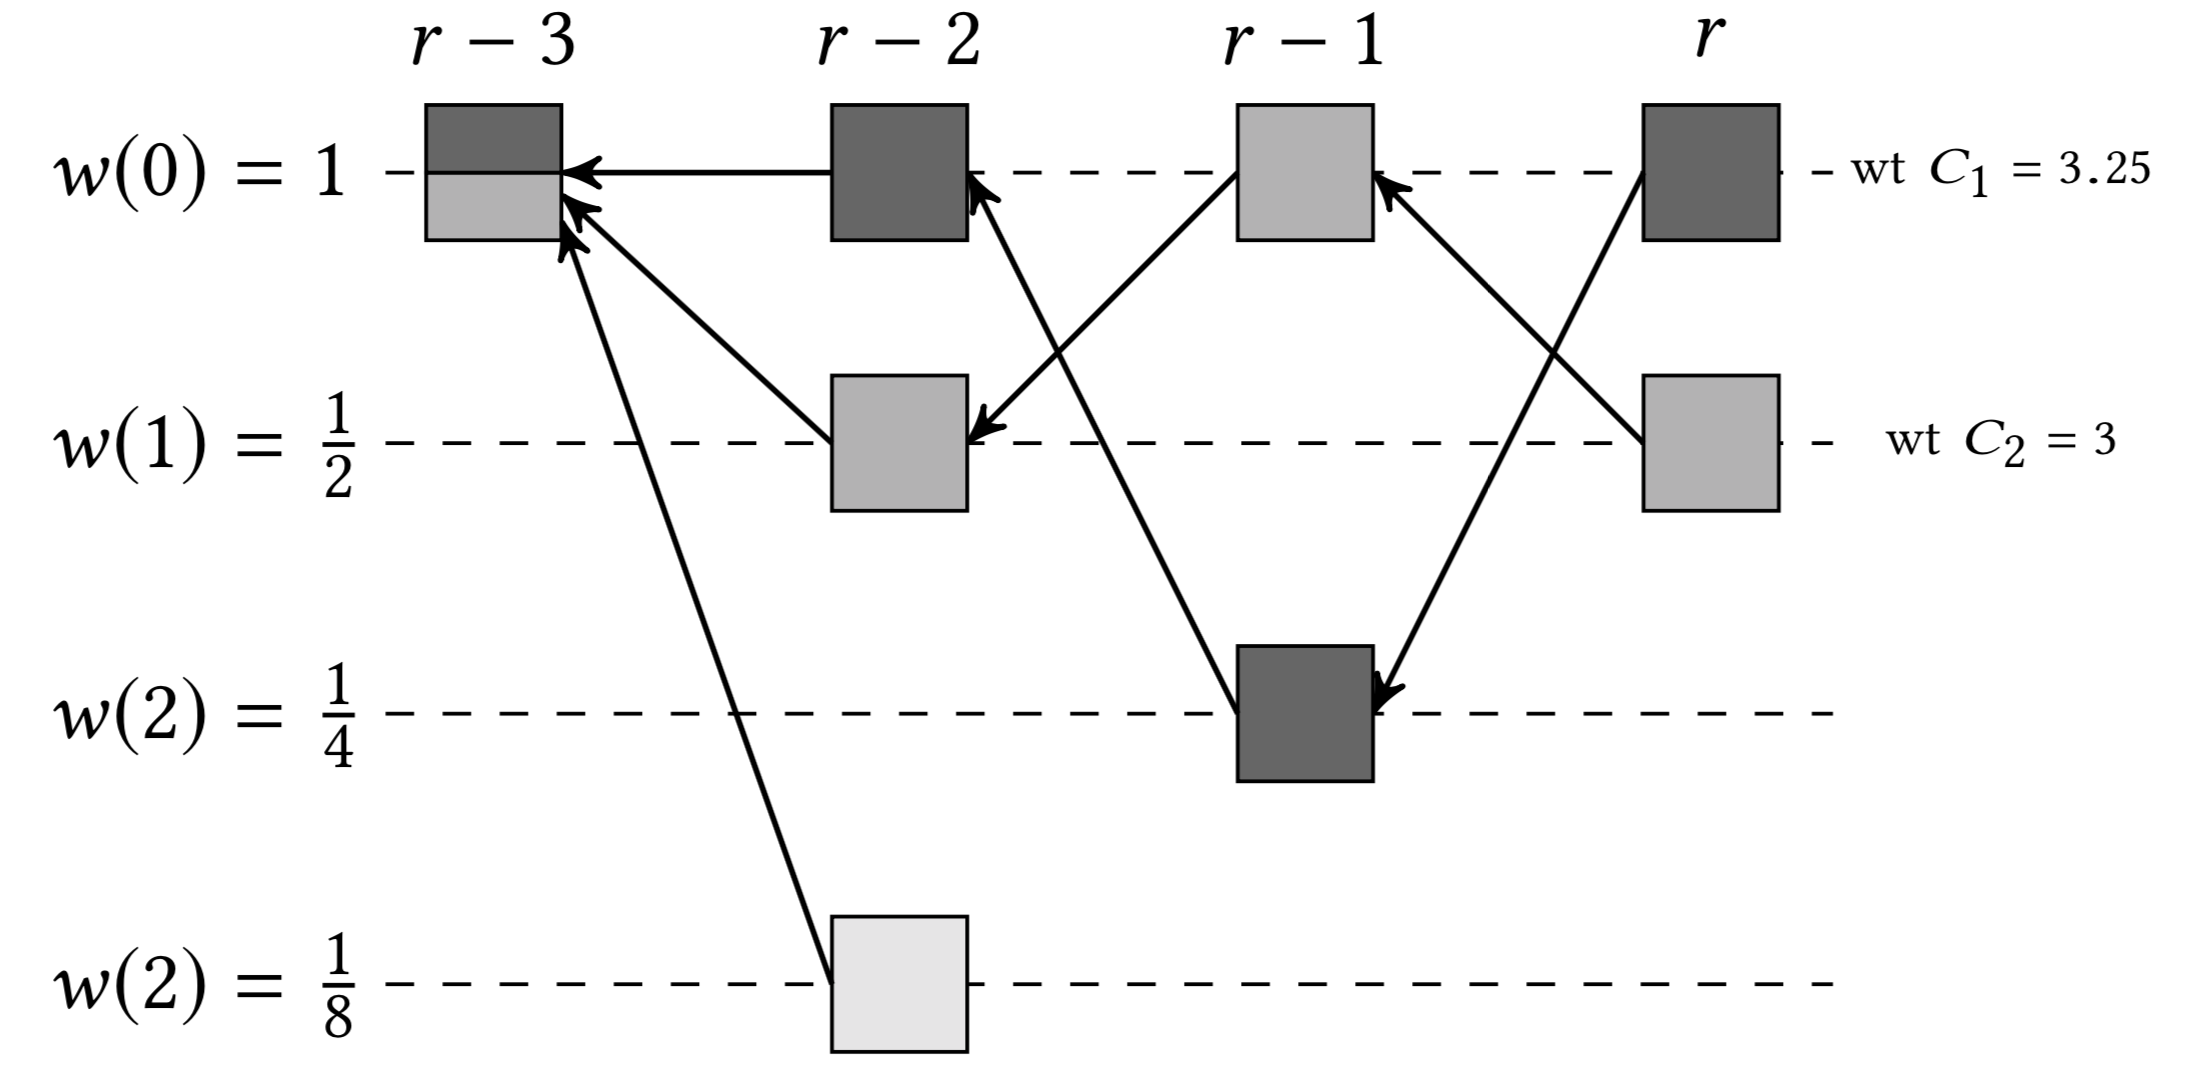
\includegraphics[width=0.8\textwidth]{../common/Dfinity_1.png}
	\caption{Dfinity区块链权重举例。四条横轴虚线对应四个矿工且权重分别为$1,1/2,1/4,1/8$。图中区块不同深浅对应与该区块属于哪一条区块链(共3条,$C_1$颜色最深,$C_3$颜色最浅)。通过计算表明链$C_1$拥有最高的总权重} 		
	\label{fig:Dfinity1}
\end{figure}
\textbf{区块提出}
矿工将区块接到权重最高的链上。注意,公证层被公证的区块仍是当前轮排名最高的区块。同时将新区块进行广播以请求公证。

\textbf{区块公证}
首先Dfinity的公证是每轮进行的。如果区块被揭露得过晚则永远不会被公证。这样有效的防止了私自挖矿(selfish mining)进攻。

一个区块被公证了当且仅当它收到了大部分公证者的签名。对每个公证者(委员会成员,也是客户端或副本节点replica),具体的公证算法用文字描述如下:
\begin{itemize}
	\item 设当前轮数为$r$。等待Blocktime时间
	\item 如果没有收到任何被公证的区块,则选择第$r$轮接收到的所有区块中排名最高的一个,对其进行签名并广播。
	\item 如果收到了被公证的区块,则$r=r+1$
\end{itemize}
文章把当前轮只有一个区块被公证的情况称作常规操作(normal operation),然后针对常规操作分析了确认时间及安全性等,但这本身是一个比较强的假设。

\textbf{最终确认}
之所以公证化不等于最终确认,是因为因传输延迟等影响存在多个区块被公证的情况。这是还需要一个最终确认(finalize)算法。

该算法描述如下:在第$r$轮,节点等待$T$时刻以接受第$r$轮被公证的区块并放入集合$N_{r}$,随后执行$Finalize(r-1)$,即,把$N_{r-1}$(即,第$r-1$轮被公正的区块集)的最长公共前缀标为最终确认。\reffig{fig:Dfinity2}指出了最终确认的过程。

同时需要基于假设:在$Finalize(h)$被执行时,$N_h$包含第$h$轮所有被公证的区块。

关于最终确认的主要定理为,在常规操作下任何交易都会在接收到两个确认信息后(被公证区块$B_r$打包,同时区块$B_{r+1}$接在上面)加上网络延迟时间的两倍内被最终确认。

\begin{figure}
	\centering
	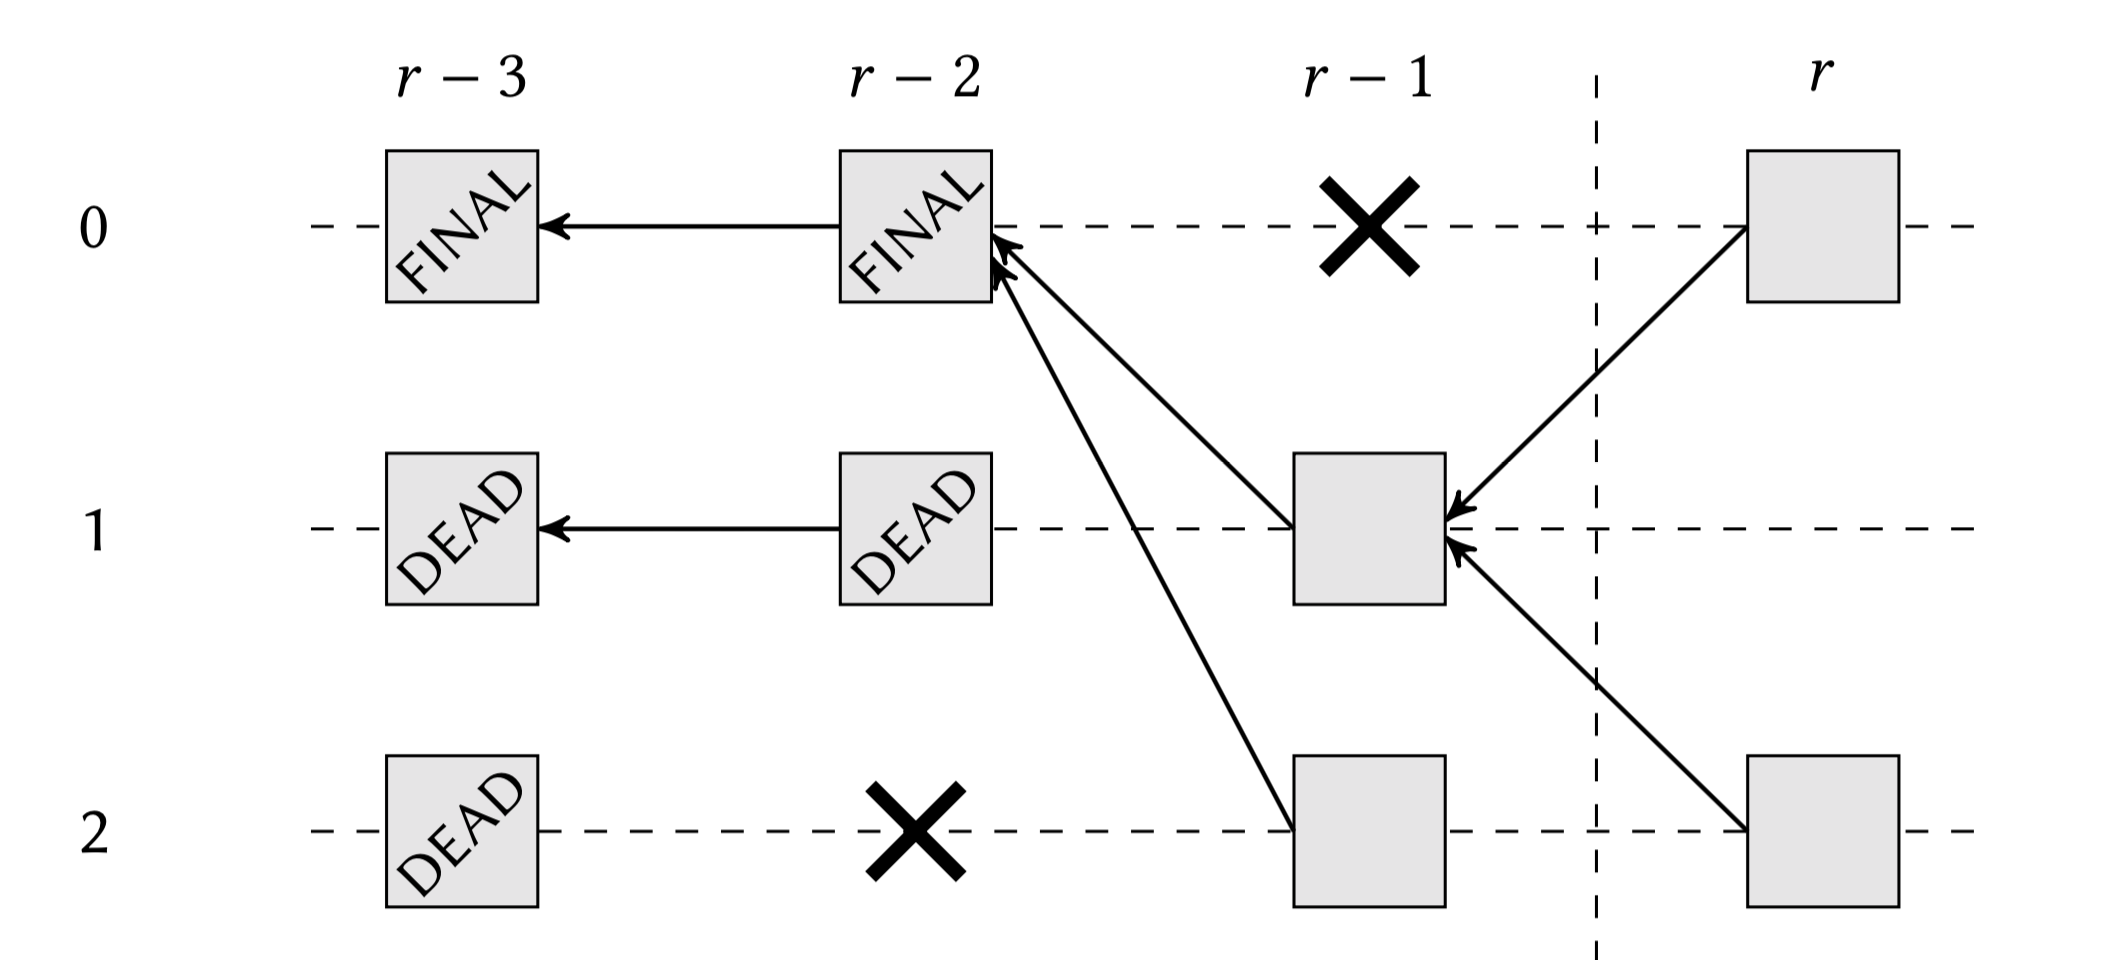
\includegraphics[width=0.8\textwidth]{../common/Dfinity_2.png}
	\caption{Dfinity区块最终确认。第$r$轮加$T$时间执行第$r-1$轮的最终确认。} 		
	\label{fig:Dfinity2}
\end{figure}

\subsection{门限签名}
关于具体原理涉及到密码学的诸多知识,这里不多做介绍。这里说明的是,$t,n$门限签名实现的主要功能为,一旦获得了$n$个人中$t$个人的签名$\sigma_{i_1},...,\sigma_{i_t}$,则可以算出所需的组签名$\sigma$。该组签名可以被任何人验证(组公钥为公开信息),且所有人的私钥仍没有被透露。其工作原理大致是用的是$t-1$次多项式函数可以被$t$个点唯一确定。

Dfinity随机种子层的工作原理就是用的门限签名。在第$r$轮开始是,每个委员会成员计算签名
$$\sigma_{r,i}=Sign(r||\xi_{r-1},sk_{G,i})$$
其中$sk_{G,i}$为成员$i$在委员会$G$中的私钥。

随后,根据$r$个签名$\sigma_{r,i}$计算出组签名$\sigma_{r,i}$,将其哈希值作为第$r$轮的输出$\xi_r$。

该签名方案简单实用,事实上被绝大部分区块链项目所使用。

Dfinity最后还提到了朝代(epoch)的概念,朝代更迭是开展对客户端/委员会候补集合的申请与注销工作。
\subsection{总结与思考}
我们认为Dfinity是一篇well written的论文,其对VRF的应用和投票思想都很清晰严谨,具有很高的借鉴意义。事实上,TAS chain白皮书\footnote{https://www.taschain.io/static/pdf/TASChainTechnologyWhitePaper.pdf}大部分就是借鉴Dfinity。不足之处在于假设过多,真正的安全性和性能存疑,而且准入门槛对于permissionless的公链也是个难以解决的问题。

%\input{economic.tex}
%%\input{nr.tex}
%\input{core.tex}
%\input{core-anti.tex}
%\input{core-impl.tex}
%\input{extension.tex}
%\input{future.tex}
%\printbibliography
\newpage
\bibliography{reference}

\newpage
%\begin{appendices}
%\input{proof}
%\input{changelog.tex}
%\end{appendices}

\end{document}
